% ------------------------------------------------------------------
%  Agenda mensuel "Surf & Armorique" - A4 portrait, 2 colonnes
%  Chaque colonne commence par un lundi.
%  Compiler avec : pdflatex agenda_mois.tex
%
%  Pour changer de mois, modifier les 4 lignes ci-dessous :
%    \moisnom    : texte affiché dans l'en-tête
%    \firstwd    : jour de la semaine du 1er du mois (1=lundi ... 7=dimanche)
%    \ndays      : nombre de jours du mois (28 à 31)
%    \firstweek  : n° de semaine ISO de la semaine contenant le 1er du mois
% ------------------------------------------------------------------
\documentclass[a4paper]{article}

\usepackage[T1]{fontenc}
\usepackage[utf8]{inputenc}
\usepackage{helvet}
\renewcommand{\familydefault}{\sfdefault}
\usepackage{xcolor}
\usepackage{tikz}
\usepackage[a4paper,left=1cm,right=1cm,top=1.2cm,bottom=1.2cm]{geometry}

\pagestyle{empty}
\setlength{\parindent}{0pt}
\setlength{\parskip}{0pt}

% --- Paramètres du mois --------------------------------------------
\newcommand{\moisnom}{OCTOBRE 2026}
\newcommand{\firstwd}{4}      % 1er octobre 2026 = jeudi
\newcommand{\ndays}{31}
\newcommand{\firstweek}{40}   % semaine ISO du lundi 28 septembre 2026

% --- Couleurs ------------------------------------------------------
\definecolor{gold}{RGB}{209,163,78}
\definecolor{navy}{RGB}{40,52,105}
\definecolor{cream}{RGB}{244,233,207}
\definecolor{paper}{RGB}{252,251,246}
\definecolor{gridgray}{RGB}{160,160,150}
\definecolor{offmonth}{RGB}{236,235,229}

% --- Noms des jours (0 = lundi ... 6 = dimanche) --------------------
\newcommand{\wdEN}[1]{\ifcase#1 MONDAY\or TUESDAY\or WEDNESDAY\or THURSDAY\or FRIDAY\or SATURDAY\or SUNDAY\fi}
\newcommand{\wdFR}[1]{\ifcase#1 LUNDI\or MARDI\or MERCREDI\or JEUDI\or VENDREDI\or SAMEDI\or DIMANCHE\fi}

\begin{document}
\noindent\makebox[0pt][l]{%
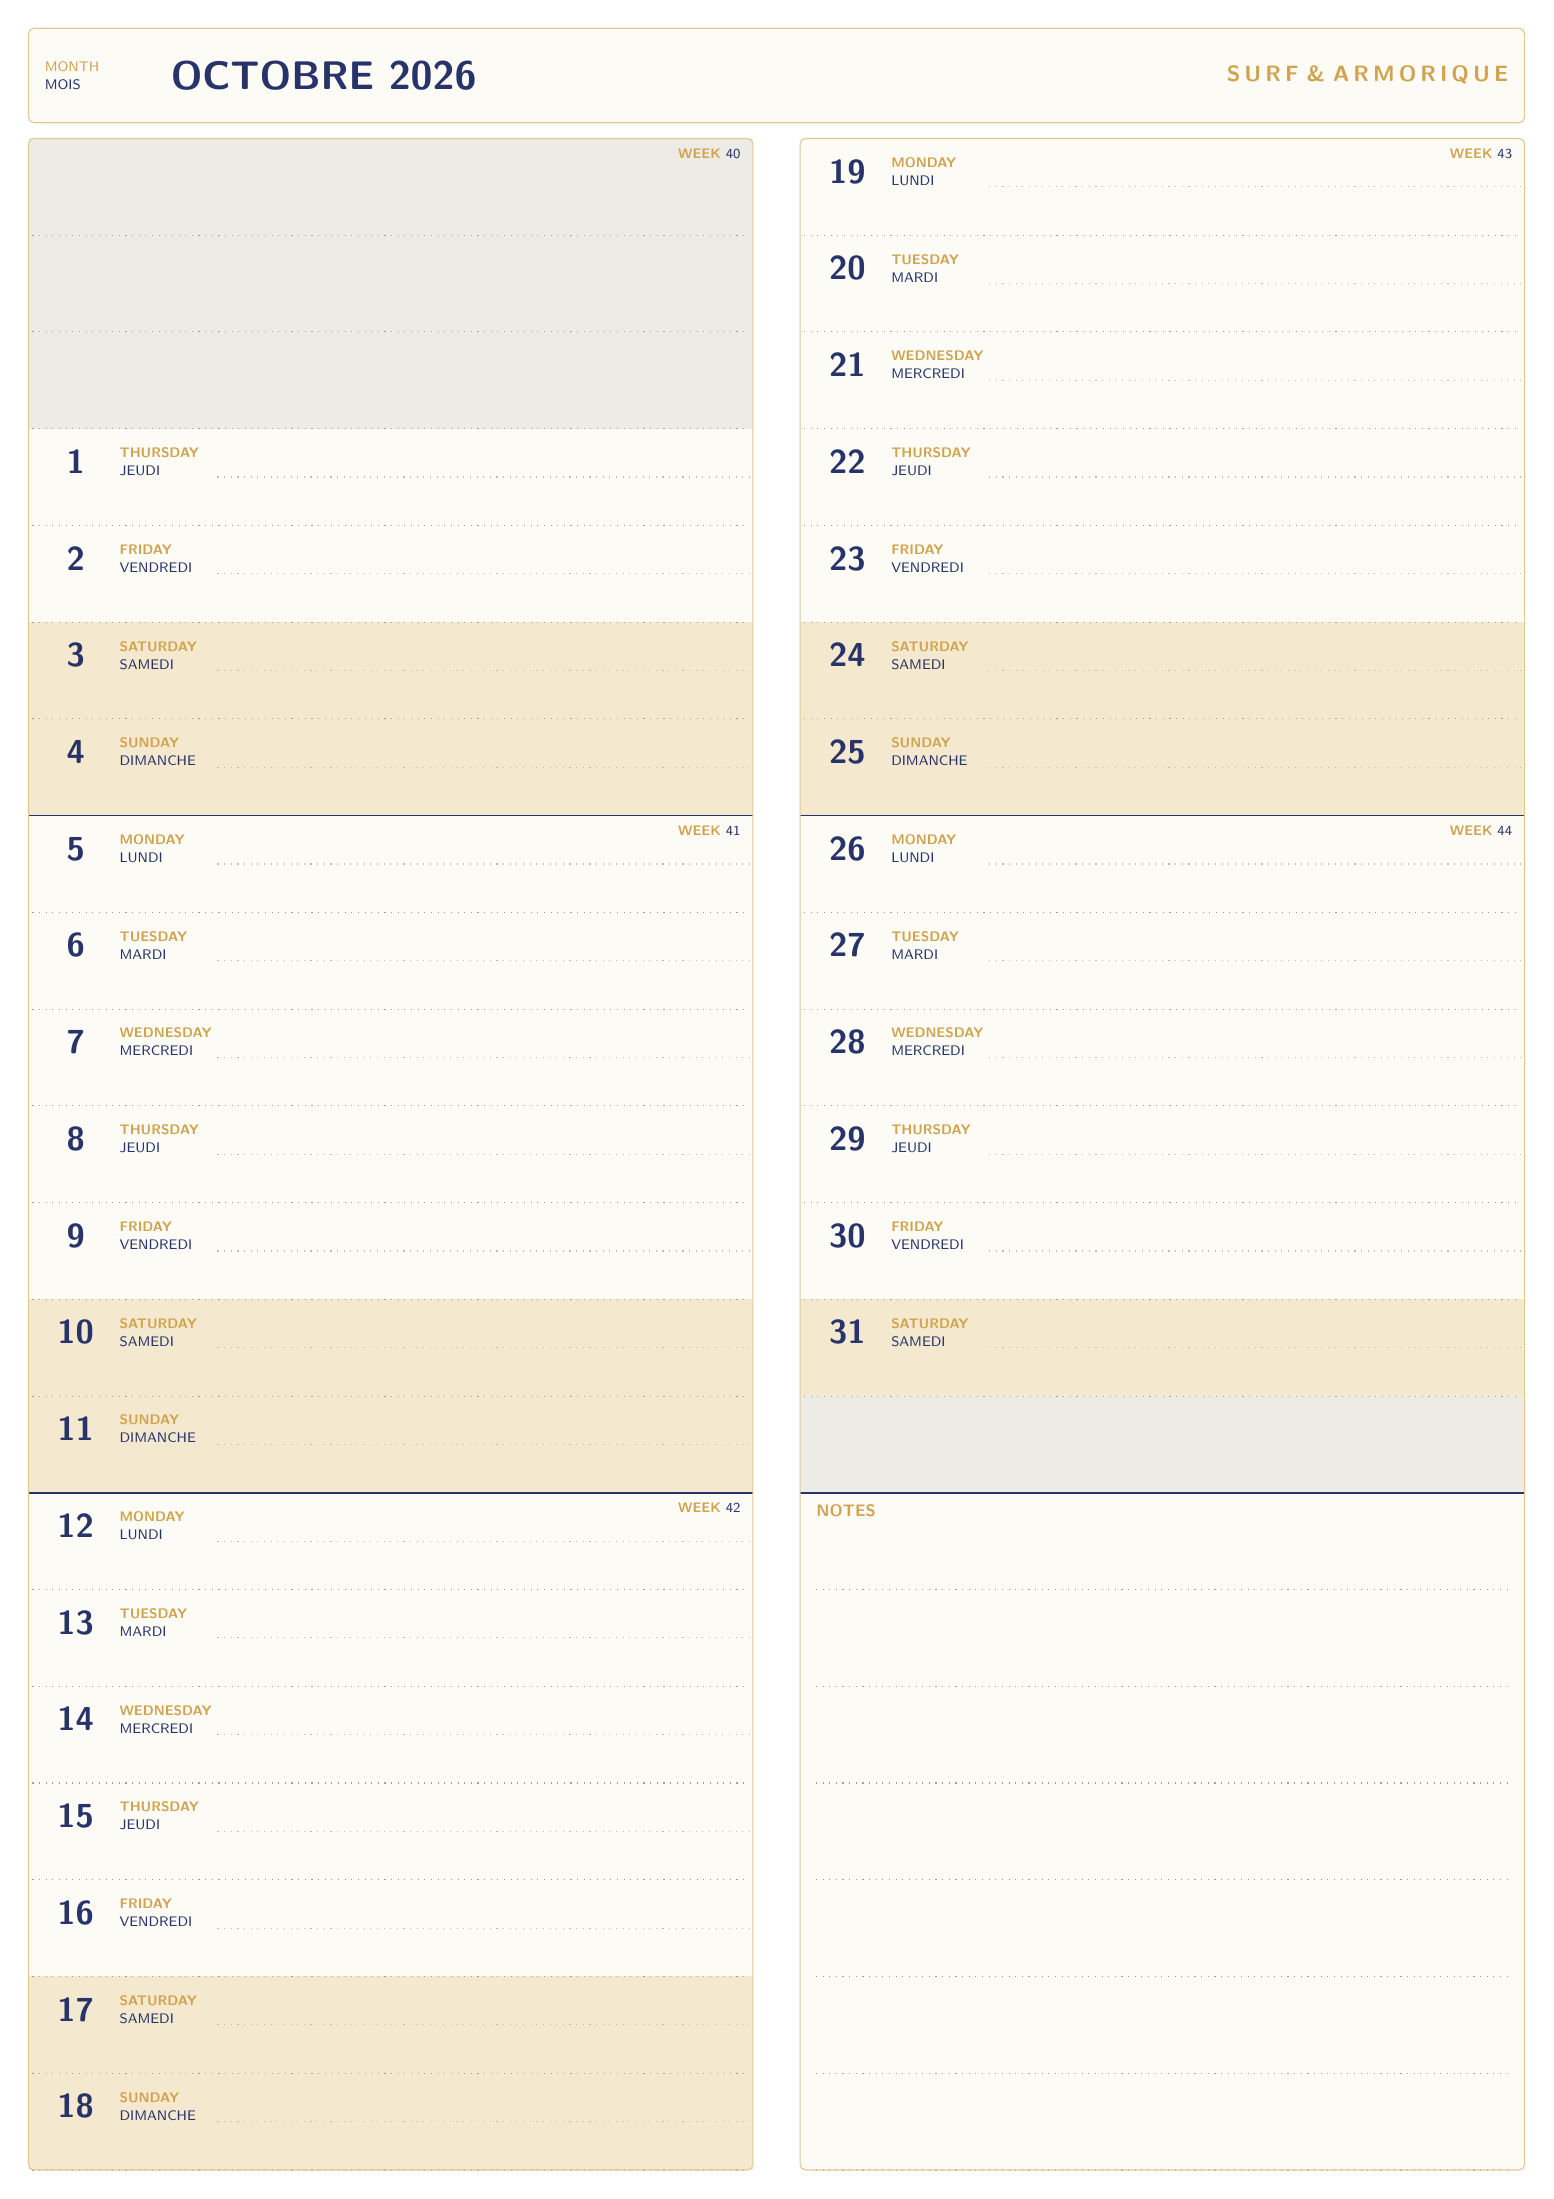
\begin{tikzpicture}[x=1cm,y=1cm]
  % --- Dimensions ---
  \def\PageW{19}
  \def\PageH{27.2}
  \def\gut{0.6}                         % espace entre les deux colonnes
  \def\hdr{1.2}                         % hauteur du bandeau d'en-tête
  \def\gap{0.2}                         % espace entre bandeau et colonnes
  \pgfmathsetmacro{\cw}{(\PageW-\gut)/2}            % largeur d'une colonne
  \pgfmathsetmacro{\ytop}{-\hdr-\gap}               % haut des colonnes
  \pgfmathsetmacro{\rh}{(\PageH-\hdr-\gap)/21}      % hauteur d'une ligne-jour (21 lignes max)

  % --- Découpage en semaines (lundi -> dimanche) ---
  \pgfmathtruncatemacro{\lead}{\firstwd-1}              % cases avant le 1er
  \pgfmathtruncatemacro{\weeks}{ceil((\lead+\ndays)/7)} % nombre de semaines
  \pgfmathtruncatemacro{\wa}{ceil(\weeks/2)}            % semaines colonne gauche
  \pgfmathtruncatemacro{\usedA}{7*\wa}                  % lignes colonne gauche
  \pgfmathtruncatemacro{\usedB}{7*(\weeks-\wa)}         % lignes colonne droite
  \pgfmathtruncatemacro{\lastcell}{7*\weeks-1}

  % --- Bandeau d'en-tête ---
  \fill[paper] (0,0) rectangle (\PageW,-\hdr);
  \draw[gold!60,line width=0.4pt,rounded corners=2pt] (0,0) rectangle (\PageW,-\hdr);
  \node[anchor=west,align=left,inner sep=0,font=\fontsize{5.5}{6.5}\selectfont]
    at (0.2,-0.6) {\textcolor{gold}{MONTH}\\\textcolor{navy}{MOIS}};
  \node[anchor=west,inner sep=0,font=\fontsize{14}{16}\selectfont\bfseries,text=navy]
    at (1.8,-0.6) {\moisnom};
  \node[anchor=east,inner sep=0,font=\fontsize{8}{9}\selectfont\bfseries,text=gold]
    at ({\PageW-0.2},-0.6) {S\,U\,R\,F\ \textbf{\&}\ A\,R\,M\,O\,R\,I\,Q\,U\,E};

  % --- Fonds des deux colonnes ---
  \foreach \cc in {0,1}{%
    \pgfmathsetmacro{\xo}{\cc*(\cw+\gut)}
    \fill[paper] (\xo,\ytop) rectangle ({\xo+\cw},{\ytop-21*\rh});
  }

  % --- Couche 1 : teintes (week-ends, jours hors du mois) ---
  \foreach \cellN in {0,...,\lastcell}{%
    \pgfmathtruncatemacro{\cc}{\cellN >= \usedA ? 1 : 0}
    \pgfmathtruncatemacro{\rowR}{\cellN-\usedA*\cc}
    \pgfmathtruncatemacro{\dayD}{\cellN-\lead+1}
    \pgfmathtruncatemacro{\wk}{mod(\cellN,7)}
    \pgfmathtruncatemacro{\valid}{(\dayD>=1 && \dayD<=\ndays) ? 1 : 0}
    \pgfmathsetmacro{\xo}{\cc*(\cw+\gut)}
    \pgfmathsetmacro{\yt}{\ytop-\rowR*\rh}
    \ifnum\valid=0
      \fill[offmonth] (\xo,\yt) rectangle ({\xo+\cw},{\yt-\rh});
    \else
      \ifnum\wk>4
        \fill[cream] (\xo,\yt) rectangle ({\xo+\cw},{\yt-\rh});
      \fi
    \fi
  }

  % --- Couche 2 : lignes, numéros, noms des jours ---
  \foreach \cellN in {0,...,\lastcell}{%
    \pgfmathtruncatemacro{\cc}{\cellN >= \usedA ? 1 : 0}
    \pgfmathtruncatemacro{\rowR}{\cellN-\usedA*\cc}
    \pgfmathtruncatemacro{\dayD}{\cellN-\lead+1}
    \pgfmathtruncatemacro{\wk}{mod(\cellN,7)}
    \pgfmathtruncatemacro{\valid}{(\dayD>=1 && \dayD<=\ndays) ? 1 : 0}
    \pgfmathtruncatemacro{\wnum}{\firstweek+int(\cellN/7)}
    \pgfmathsetmacro{\xo}{\cc*(\cw+\gut)}
    \pgfmathsetmacro{\yt}{\ytop-\rowR*\rh}
    \pgfmathsetmacro{\yb}{\ytop-(\rowR+1)*\rh}
    \pgfmathsetmacro{\ym}{\ytop-(\rowR+0.5)*\rh}
    % ligne de séparation pointillée en bas de la ligne
    \draw[gridgray,dotted,line width=0.4pt] ({\xo+0.05},\yb) -- ({\xo+\cw-0.05},\yb);
    \ifnum\valid=1
      % ligne d'écriture intermédiaire
      \draw[gridgray!70,dotted,line width=0.4pt] ({\xo+2.4},\ym) -- ({\xo+\cw-0.05},\ym);
      % numéro du jour
      \node[inner sep=0,font=\fontsize{12}{13}\selectfont\bfseries,text=navy]
        at ({\xo+0.6},{\yt-0.42}) {\dayD};
      % nom du jour (EN doré / FR bleu)
      \node[anchor=west,align=left,inner sep=0,font=\fontsize{5.5}{6.5}\selectfont]
        at ({\xo+1.15},{\yt-0.42}) {\textcolor{gold}{\bfseries\wdEN{\wk}}\\\textcolor{navy}{\wdFR{\wk}}};
    \fi
    % début de semaine : trait plein + numéro de semaine
    \ifnum\wk=0
      \ifnum\rowR>0
        \draw[navy,line width=0.6pt] (\xo,\yt) -- ({\xo+\cw},\yt);
      \fi
      \node[anchor=north east,inner sep=0,font=\fontsize{5}{6}\selectfont]
        at ({\xo+\cw-0.15},{\yt-0.12}) {\textcolor{gold}{\bfseries WEEK}\ \textcolor{navy}{\wnum}};
    \fi
  }

  % --- Zone NOTES dans l'espace libre de chaque colonne ---
  \foreach \cc/\used in {0/\usedA,1/\usedB}{%
    \ifnum\used<21
      \pgfmathsetmacro{\xo}{\cc*(\cw+\gut)}
      \pgfmathsetmacro{\yt}{\ytop-\used*\rh}
      \draw[navy,line width=0.6pt] (\xo,\yt) -- ({\xo+\cw},\yt);
      \node[anchor=north west,inner sep=0,font=\fontsize{6}{7}\selectfont\bfseries,text=gold]
        at ({\xo+0.2},{\yt-0.15}) {NOTES};
      \pgfmathtruncatemacro{\nextrow}{\used+1}
      \foreach \rr in {\nextrow,...,21}{%
        \pgfmathsetmacro{\yy}{\ytop-\rr*\rh}
        \draw[gridgray,dotted,line width=0.4pt] ({\xo+0.2},\yy) -- ({\xo+\cw-0.2},\yy);
      }
    \fi
  }

  % --- Contours des colonnes ---
  \foreach \cc in {0,1}{%
    \pgfmathsetmacro{\xo}{\cc*(\cw+\gut)}
    \draw[gold!60,line width=0.4pt,rounded corners=2pt]
      (\xo,\ytop) rectangle ({\xo+\cw},{\ytop-21*\rh});
  }
\end{tikzpicture}}\par
\end{document}
